\documentclass[12pt, a4paper, twocolumn]{article}
%\documentclass[10pt]{article}
\usepackage[english]{babel}
\usepackage{graphicx}
\usepackage{float}
\usepackage{multirow}
\usepackage{caption} 
\usepackage{subcaption} 
\usepackage[T1]{fontenc}
\usepackage[utf8]{inputenc}
\usepackage{authblk}
%\usepackage{setspace}
\usepackage[margin=1in]{geometry}
\usepackage{abstract}
\usepackage{fancyhdr}
%\setlength{\headheight}{15.2pt}
\pagestyle{fancyplain}
\usepackage[utf8]{inputenc}
\usepackage[T1]{fontenc}
\usepackage{cite}
\usepackage{amssymb}
\usepackage{amsmath}
\usepackage{ulem}

\begin{document}

\fancyhf{}
\lhead{CHEG 827}
\rhead{\thepage}
%\rfoot{\fancyplain{}{\thepage}}

\title{Lanczos Iteration Applied to the Variational Method in Quantum Mechanics}

\author[1]{Marcel P. N\'{u}\~{n}ez\thanks{mpnunez@udel.edu}}
\affil[1]{University of Delaware, Newark, DE}

\date{\today}

\twocolumn[

\maketitle

\begin{center}
\line(1,0){450}
\end{center}

\begin{onecolabstract}

Approximate solutions to the Schr$\ddot{\mathrm{o}}$dinger equation are found using the variational method and a plane wave basis set. This method is used for a single electron in a periodic cell subject to an arbitrary potential. Use of a basis set converts the problem from a continuum one solving for an eigenfunction into a simpler discrete problem solving for an eigenvector. The components of the eigenvector of a matrix give contributions of each basis function to the solution wavefunction. Matrix formulation allows the use of highly developed machinery for efficiently finding the eigenvalues and eigenvectors of large matrices. In this way, more basis functions can be used, which provides a better approximation of the solution. In this work we are working with a large symmetric matrix, so Lanczos iteration is used. It is found that use of the Lanczos algorithm accelerates the task of diagonalizing the Hamiltonian matrix, which is the slowest part of the computation.
\\{\bf Keywords:} Lanczos algorithm, fast Fourier transform, quantum mechanics
\end{onecolabstract}

\begin{center}
\line(1,0){450}
\end{center}

]

\saythanks

\onecolumn

%
%\tableofcontents
%
%\newpage
%
%\twocolumn

\section{Introduction}%motivation and historical development

Catalysis research requires understanding interactions between molecules or between molecules and a catalyst surface. The nature of this interaction is electronic. Density functional theory, the development of which earned the 1998 Nobel Prize in Chemistry, computes electronic structure from first principles. 

Numerically, it is an iterative method that computes the electron cloud density by using a functional of the density to compute an effective potential in a self-consistent field (SCF) calculation. The solution to the SCF is obtained from a quantum mechanical calculation for a single electron. It decouples the interactions between electrons and solves the Kohn-Sham equation, so that for electron $i$

\begin{equation}
\left( - \frac{\hbar ^2}{2m} \nabla ^2 + v_{\mathrm{eff}} \right) \psi_i (r) = \epsilon_i \psi_i (r)
\end{equation}
 
Contributions to the effective potential $v_{\mathrm{eff}}$ are elctron-nuclear coulombic interactions, electron-electron coulombic interactions, and exchange correlation which captures the Pauli-exclusion princple and spin. Typically, the hartree-Fock approximation, which approximates the wavefunction for a single electron as a slater determinant of single-electron orbitals, is used to ensure the satisfaction of the Pauli-exclusion principle. In this work we do only single electron calculations, so we do not need to invoke this. 

For any system more complex than the hydrogen atom, no analytical solution exists. A computational algorithm for finding the solution to the Kohn-Sham equation then becomes necessary. 

At a basic level we need to be able to solve the time independent Schrondinger equation for a single electron. In principle we could discretize our space and solve the nonlinear partial differential equation. However, an easier way to arrive at the solution is to use the variational method, which approximates the wavefunction as a linear combination of an orthonormal set of basis functions. 


In Section \ref{sec:var} we present the variational approach in quantum mechanics. In Section \ref{sec:nummeth} we discuss the numerical methods used to speed up the computational implementation of the variational method. In Section~\ref{sec:modval} we validate our approach by solving the one-dimensional quantum harmonic oscillator and compare the results to the analytical solution. In Section \ref{sec:cpu} we analyze the CPU requirements of each portion of the algorithm to identify the bottleneck. Finally, in Section \ref{sec:conc} we summarize the major conclusions of our investigation.

\section{Variational Approach}
\label{sec:var}


We want to get an accurate approximation of our wavefunction by using a large number of basis functions. In addition, the contributions of different basis functions will tell us the character of our wavefunction.

The first thing to do is to choose a set of basis functions $\{ \phi_i \}$ which satisfy the orthonormality condition

\begin{equation}
\int_V \phi_i^*\phi_j dV = \delta_{ij}.
\end{equation}

We can the express the solution wavefunction as 

\begin{equation}
\Psi = \sum_i c_i \phi_i 
\end{equation}

subject to the normalization condition 

\begin{equation}
\sum_i |c_i|^2 = 1.
\end{equation}

Then we solve for the values of $\{ c_i \}$ which make $\Psi$ an eigenfunction of the Hamiltonian operator. The problem can be transformed to a linear one by expressing the function $\Psi$ as the vector $\uline{\Psi}$ containing the coefficients  $\{ c_i \}$. Likewise, the Hamiltonian operator can be expressed as a matrix

\begin{equation}
\uuline{\hat{H}}_{i,j} = \int_V \phi_{i} ^* \hat{H} \phi_{j} dV
\end{equation}

which contains all the information about how the Hamiltonian of the system operates on the set of basis functions. Solving Schroniger equation becomes a problem of finding the eigenvalues of the Hamiltonian matrix. This is advantageous because there exists a wealth of machinery to deal with linear problems. Notice that because $\hat{H}$ is a Hermetian operator, the matrix $\uuline{\hat{H}}$ is a Hermetian matrix.

The energy of a solution is 

\begin{equation}
E_n = \frac{ \uline{\Psi}_n ^* \cdot \uuline{\hat{H}} \cdot \uline{\Psi}_n }{ \uline{\Psi}_n^* \cdot \uline{\Psi}_n }.
\end{equation}

%\begin{equation}
%E = \frac{\int_{V} \Psi^* \hat{H} \Psi dV}{\int_V \Psi^* \Psi dV}
%\end{equation}

where $E_n$ is the eigenvalue corresponding to the eigenvector $\uline{\Psi}_n$. The variational method is good for approximating the few lowest energy states of the system. So we can find the few smallest eigenvalues and eigenvectors which will approximate the ground state and lowest excited states of the system.

\subsection{Plane-Wave Basis Set}

The basis wave function we will use is the plane wave basis. The motivation behind plane-waves is that taking derivatives and integrals is extremely easy, so it will not be necessary to do these numerically. They work especially well in systems with periodic potentials, such as crystals. This is expressed in Bloch Theorem. Use of plane waves requires restricting our problem to a periodic cell $V$. If $V$ is a parallelogram whose edges are the vectors $a_1$, $a_2$, and $a_3$, then we can construct the reciprocal lattice vectors $b_1$, $b_2$, and $b_3$, which satisfy

\begin{equation}
a_{i}\cdot b_{j} = 2\pi\delta_{ij}
\end{equation}

This allows us to define a plane wave basis set, each element of which is defined by three positive integers $i$, $j$, and $k$. It is a spatial Fourier transform defined by the equation


\begin{equation}
\phi_{ijk}= \frac{1}{\sqrt{\Omega}} e^{iG_{ijk}\cdot r}
\end{equation}

where $\Omega=a_1\cdot(a_2\times a_3)$ is the volume of $V$ and
$G_{ijk} = ib_1 + jb_2 + kb_3$ is a vector connecting two points on the reciprocal lattice. Just as Fourier components with different frequencies are orthonormal, so are plane waves. This basis also has some good analytical simplifications that will allow us to quickly compute the matrix $\uuline{H}$. In particular, the Kinetic energy of a plane-wave is 

\begin{equation}
\int_{V} \phi_{ijk}^* \left( -\frac{\hbar^2}{2m}\nabla ^2 \phi_{ijk}\right) dV = \frac{\hbar^2}{2m} |G_{ijk}|^2.
\end{equation}

This will allow us to completely solve the problem without ever having to evaluate the second derivative numerically. It also gives a good way to choose a finite basis set. Typically The basis set is restricted by including only those plane-waves whose kinetic energy lies below a cutoff $E_{\mathrm{cut}}$.

Plane-waves are orthogonal with respect to the kinetic energy operator. A typical assumption is that the kinetic energy and potential energy contributions to the Hamiltonian are separable. Therefore, the matrix $\uuline{H}$ can be decomposed into 

\begin{equation}
\uuline{\hat{H}} = \uuline{\hat{H}}_{\mathrm{KE}} + \uuline{\hat{H}}_{\mathrm{PE}}
\end{equation}

where 

\begin{equation}
\uuline{\hat{H}}_{\mathrm{KE},ij} = \left\{
     \begin{array}{lr}
       \frac{\hbar^2}{2m} |G_{ijk}|^2 & : i = j\\
       0 & : i \neq j
     \end{array}
   \right.  
\end{equation}

and

\begin{equation}
\uuline{\hat{H}}_{\mathrm{PE},ij} = \int_V \phi_{ijk}^* \hat{V} \phi_{ijk} dV.
\end{equation}

This matrix has nonzero offdiagonal terms. The potential inside the box will cause different basis wavefunctions to blend. Computing $\uuline{H}_{\mathrm{PE},ij}$ will require spatial integrations, but this can be made faster with Fourier transform. That's because we can express our potential as 

\begin{equation}
	\hat{V}(r) = \sum_{ijk} \nu (i,j,k) e ^ {i G_{ijk} \cdot r}
\end{equation} 

then the matrix element is just one component of the Fourier series

\begin{equation}
\uuline{\hat{H}}_{\mathrm{PE,ij}} = \int_V \sum_{ijk} \nu (i,j,k) e ^ {i G_{ijk} \cdot r} \frac{1}{\Omega} e^{i (G_{ijk} - G_{ijk})\cdot r} dV = \nu(\Delta i,\Delta j, \Delta k)
\end{equation}


\section{The Lanczos Algorithm}
\label{sec:nummeth}

The Lanczos algorithm is a simplified Arnoldi method. The Arnoldi algorithm generates an orthonormal basis of the Kyrlov subspace and uses it to compute approximations of the eigenvectors with the $r$ largest eigenvalues. It does this by using the basis of the Kyrlov subspace to transform the matrix $A$ into a matrix of smaller dimension. If $A$ is an $n$ by $n$ matrix, $b$ is the initial guess of the eigenvector, and we have $r<<n$, then

\begin{equation}
K_r(A,b) = \mathrm{span} \{b,Ab,A^2 b,\cdots ,A^{r-1}b\}
\end{equation}

This iteration is unstable, so instead we compute an orthonormal basis for the Kyrlov subspace $\{q_1,\cdots , q_r \}$. $q_1=b$ which is a random vector of norm one. After that, All of the vectors are orthogonalized against all the previous ones. Make a matrix $V_{[n\times r]}=[q_1,\cdots,q_r]$ of the Krylov subspace basis. We can also make the upper Hessenberg matrix

\begin{equation}
H_{[r\times r]}=V^*AV
\end{equation}

for which 

\begin{equation}
H_{ij} = q_i^*Aq_j
\end{equation}

The orthonormalization of the vectors $\{q_i\}$ makes $H$ an upper Hessenberg matrix. If $A$ is Hermetian, then $H$ is tridiagonal and we use a different notation to capture this important feature

\begin{equation}
T_{mm}=V_m^* A V_m.
\end{equation}

This makes the calculation of $H$ much easier since there are now $N+2(N-1)=3N-2$ nonzero terms rather than $\frac{1}{2}N(N-1)$. Additionally, we must find the eigenvalues and eigenvectors of $H$ with some more computationally intensive but more accurate method, such as the QR algorithm. This will be easy becaues $H$ is of modest size, having dimensions $r \times r$ rather than $n \times n$. The eigenvalues of $H$ approximate the $r$ eigenvalues of $A$ with the greatest magnitudes. Additionally, if $v_i$ is an eigenvector of $H$ then $Vv_i$ gives an approximation of the corresponding eigenvalue of $A$.

\section{Model Validation}
\label{sec:modval}

Look at the one-dimensional quantum harmonic oscillator. This is one of the few problems for which an analytical result exists. The potential energy operator in a harmoic oscillator system is 

\begin{equation}
\hat{V} = \frac{1}{2}kx^2=\frac{1}{2}m\omega^2x^2
\end{equation}

where $k$ is the spring constant, $\omega = \sqrt{\frac{k}{m}}$ is the frequency, and $x$ is the distance from the equilibrium position. Plugging this into Schrodinger's Equation, it becomes

\begin{equation}
\hat{H} = -\frac{\hbar^2}{2m} \frac{\delta^2}{\delta x^2} +\frac{1}{2}m\omega ^2 (x-x_{\mathrm{eq}}).
\end{equation}

\begin{table}[t]\footnotesize
	\centering
	\caption{Physical parameters used for quantum harmonic oscillator.}
	\begin{tabular}{| c | c | c | c |}
	\hline
    Variable & Symbol & Value \\
    \hline 
    Box length & $L$ & $2\cdot 10^{-10} \mathrm{m}$ \\
    \hline 
    Frequency & $\omega$ & $5.63212\cdot 10^{14} \mathrm{s}^{-1}$ \\
    \hline 
    Electron reduced mass & $m$ & $1.62661\cdot 10^{-27} \mathrm{Kg}$ \\
    \hline 
    Plank's constant & $\hbar$ & $1.054571\cdot 10^{-34} \mathrm{Js}$ \\
    \hline
  \end{tabular}
\label{tab:physparam}
\end{table}

The analytical solution is

\begin{equation}
\Psi_n(x) = \frac{1}{\sqrt{2^m n!}} \left( \frac{m \omega}{\pi \hbar} \right)^{\frac{1}{4}} e^{ -\frac{m\omega x^2}{2\hbar} }H_n \left( \sqrt{\frac{m \omega}{\hbar}}x \right)
\end{equation}

where $H_n$ is the Hermite polynomial of order $n$.

The associated energy levels are 

\begin{equation}
E_n = \hbar \omega (n+\frac{1}{2})
\end{equation}

We evaluate the solution in a box ranging from $x=-\frac{L}{2}$ to $x=\frac{L}{2}$. Values of the physical parameters are shown in Table \ref{tab:physparam}. In Figure \ref{fig:a1} we have plotted the analytical solution for the ground state wavefunction against the one obtained using the variational method. As more plane waves are used to approximate the solution wavefunction, the numerical solution becomes closer to the analytical one. 

\begin{figure}[h!]
  \centering
    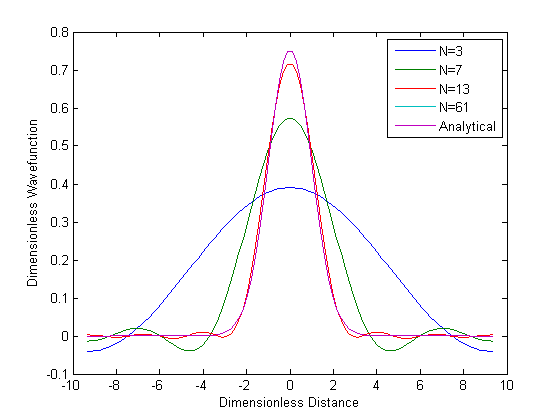
\includegraphics[scale=0.5]{a1.png}
	\caption{Comparison of numerically obtained solution for the quantum harmonic oscillator with the analytical solution. Lengths are divided by $\sqrt{\frac{\hbar}{m\omega}}$ to obtain dimensionless values.}
	\label{fig:a1}
\end{figure}

We can also plot the energies at each energy state for the analytical and numerical solutions in Figure \ref{fig:a2}. We see that when 60 basis functions are used, approximately the first 30 are accurate. The inaccuracy of the highest excited states is due to the failure of the variational method for excited states.

\begin{figure}[h!]
  \centering
    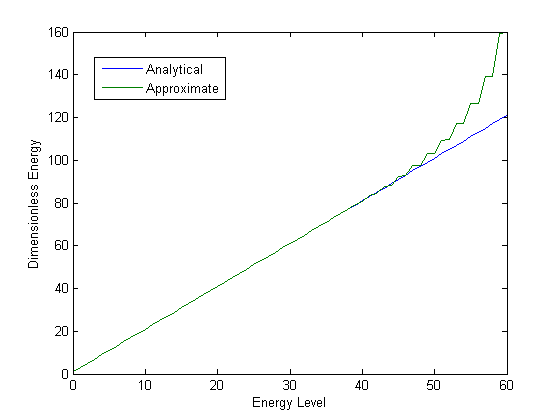
\includegraphics[scale=0.5]{a2.png}
	\caption{Comparison of numerically obtained energies for the quantum harmonic oscillator with the analytical solution. Energies are divided by $\frac{\hbar\omega}{2}$ to obtain dimensionless values. An energy level is 0 is the ground state. 61 plane waves are used.}
	\label{fig:a2}
\end{figure}

The coefficients of the ground state eigenvector show which basis wavefunctions contribute the most to the solution. We we graphically that about the first 15 are important.

\begin{figure}[h!]
  \centering
    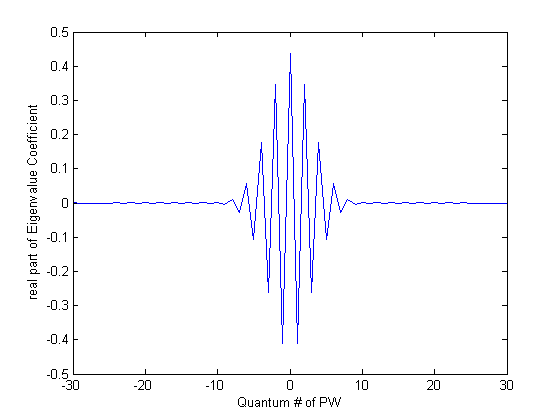
\includegraphics[scale=0.5]{a3.png}
	\caption{Values of the coefficients of each plane wave. 61 plane waves are used.}
	\label{fig:a3}
\end{figure}



\section{Error Behavior and Speed}
\label{sec:cpu}

The error in the approximation of the ground state energy verses the number of basis functions used is shown in Figure \ref{fig:a4}. The error decreases exponentially with the number of basis functions used in two regimes. The dependence is steep, so that the numerical accuracy reaches the highest accuracy obtainable with the variational principle by approximately 35 basis functions.

\begin{figure}[h!]
  \centering
    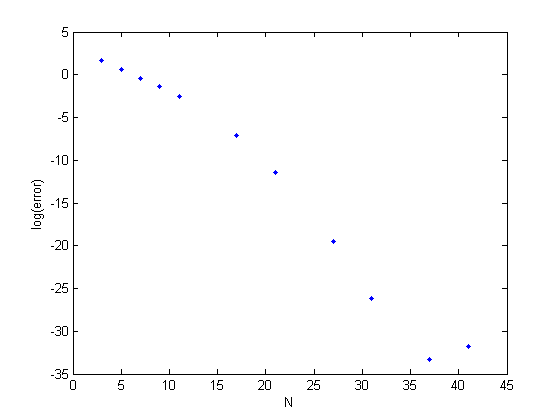
\includegraphics[scale=0.5]{a4.png}
	\caption{Error behavior of the solution against number of plane waves used in the calculation.}
	\label{fig:a4}
\end{figure}

There are two intensive parts of solving this problem. The first is taking the Fourier transform of the potential. The second is finding the eigenvalues of the Hamiltonian matrix. Figure \ref{fig:s1} shows the CPU time requirements of each step of the calculation. Both methods for finding the eigenvalues are shown.

\begin{figure}[h!]
  \centering
    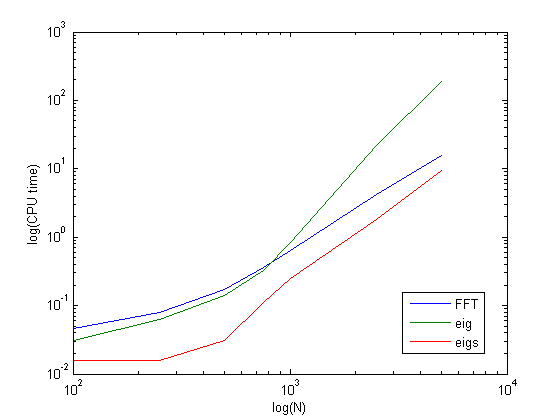
\includegraphics[scale=0.5]{s1.png}
	\caption{CPU time requirements for various parts of the calculation.}
	\label{fig:s1}
\end{figure}

With higher dimensionality, the Fourier transform requires more time. The time required to find the eigenvalues depends on only on the size of the matrix $\uuline{H}$, which is the number of basis functions we use. There is a question of how many basis functions need to be used to get an accurate solution to the problem.

Figure \ref{fig:s2} shows the time requirements for using the Lanczos Algorithm to compute more excited state. Because it is an iterative method, the time requirement increases linearly with $k$. However, the relation is slightly more than linear because of the increased computational load associated with orthonormalizing basis vectors of the Krylov subspace against previous ones.

\begin{figure}[h!]
  \centering
    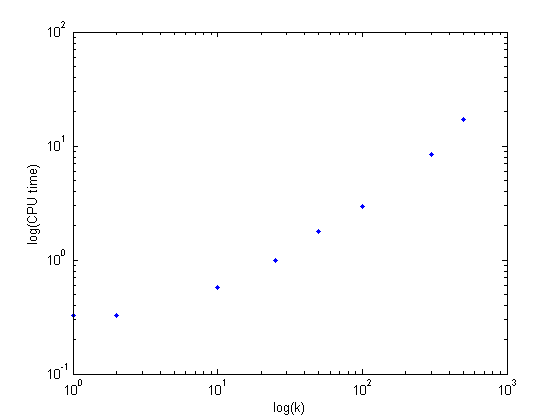
\includegraphics[scale=0.5]{s2.png}
	\caption{CPU time requirements for obtaining multiple eigenvalues with Lanczos iteration.}
	\label{fig:s2}
\end{figure}

\section{Conclusions}
\label{sec:conc}

The variational method in quantum mechanics has been cast in a form able to be solved with matrix methods. The Lanczos Algorithm was chosen to accelerate the computationally limiting task of finding the eigenvalues and eigenvectors of the Hamiltonian matrix. It is found that the Lanczos algorithm is appropriate because only the smallest eigenvalues are of physical relevance when employing the variational method. The speed of the Lanczos method is somewhat slowed by having to work implicitly with the inverse of the Hamiltonian matrix to access the smallest eigenvalues. 


%\begin{thebibliography}{9}

%\bibitem{ESM}
%  Haar, D. \textit{Elements of Statistical Mechanics}, $3^{\mathrm{rd}}$ ed.; Butterworth-Heinemann Ltd, 1995.


%1.	NUMERICAL SOLUTION OF THE KOHN-SHAM EQUATION BY FINITE ELEMENT METHODS WITH AN ADAPTIVE MESH REDISTRIBUTION TECHNIQUE GANG BAO†‡, GUANGHUI HU†, AND DI LIU†
%2.	Numerical methods for electronic structure calculations of materials ¤Yousef Saad † James R. Chelikowsky‡ Suzanne M. Shontz
%3.	That class in Italy on numerical methods in quantum mechanics
%4.	Quantum Chemistry textbook

%\end{thebibliography}

\end{document}
